 \section{Case Studies}
\label{sec:case_study}
To demonstrate the effectiveness of the Safety Annex, we describe two case studies.



\iffalse
\subsection{Simple Wheel Brake System}
The Wheel Brake System (WBS) described in ARP4761 has been used as a case study for safety analysis, formal verification, and contract based design in numerous studies. In order to show scalability compare results with other tools and studies, the AADL model of the WBS used in~\cite{Stewart17:IMBSA} was enhanced using as a guide the NuSMV ARCH4 model as described in~\cite{DBLP:conf/cav/BozzanoCPJKPRT15}. This version of the WBS model was chosen due to the complexity of the model and because this model addresses required safety concerns (for description of these concerns, see~\cite{DBLP:conf/cav/BozzanoCPJKPRT15}). Due to the added complexity of this WBS system, a short description of the subcomponents and behavior is necessary.

\subsubsection{Simple WBS architecture description}
The highest level model component is the WBS. It consists of the Braking System Control Unit (BSCU), green and blue hydraulic pressure lines (supplied by the green and blue hydraulic pumps respectively), a selector which selects between normal operating mode and alternate operating mode, and the wheel system.

There are three operating modes of the WBS. In \textit{normal} mode, the system uses the \textit{green} hydraulic circuit. In \textit{alternate} mode, the system uses the \textit{blue} hydraulic circuit.  If the BSCU detects lack of pressure from the green line or one of its command units are invalid, then the system switches into alternate mode. The last mode of operation of the WBS is the \textit{emergency} mode. This is supported by the blue circuit but operates if the blue hydraulic pump fails. The accumulator pump has a reserve of pressurized hydraulic fluid and will supply this to the blue circuit in emergency mode.  Antiskid braking commands receive data from the BSCU that will determine if skidding is found at the wheel and handle accordingly.

In the simplified WBS model, there is one wheel that receives pressure from either the green or blue line. This wheel provides feedback to the BSCU providing information about the pressure supplied.

To evaluate the effectiveness of the Safety Annex, we updated the simple WBS model~\cite{Stewart17:IMBSA} to specify faulty component behaviors. The components' nominal  and faulty behaviors are modeled separately. At the top-level AADL component, the fault hypothesis was specified as the maximum number of faults that can be active at any time. The AGREE contracts at the top-level component were verified using AGREE, with the ``Perform Safety Analysis'' option selected. This signals the tool to weave the nominal and faulty behaviors into one augmented AGREE model before feeding to the model checker.

In this example, the top level contract ``Pedal pressed and no skid implies brake pressure applied'' was verified in the presence of at most one fault active during execution.  However, it was shown to be invalid when more than one fault was allowed. The counterexample indicated that both Selector's outputs failed to non-deterministic values due to the faults introduced.
\fi


\subsection{Wheel Brake System}
%original in the case study:
%The Wheel Brake System (WBS) described in ARP4761 has been used as a case study for safety analysis, formal verification, and contract based design in numerous studies. In order to show scalability compare results with other tools and studies, the AADL model of the WBS used in~\cite{Stewart17:IMBSA} was enhanced using as a guide the NuSMV ARCH4 model as described in~\cite{DBLP:conf/cav/BozzanoCPJKPRT15}. This version of the WBS model was chosen due to the complexity of the model and because this model addresses required safety concerns (for description of these concerns, see~\cite{DBLP:conf/cav/BozzanoCPJKPRT15}). Due to the added complexity of this WBS system, we provide a short description of the subcomponents and behavior.
%from related work:
%The Wheel Brake System (WBS) described in ARP4761~\cite{SAE:ARP4761} has been used in the past as a case study for safety analysis, formal verification, and contract based design~\cite{DBLP:conf/cav/BozzanoCPJKPRT15, 10.1007/978-3-319-11936-6-7, CAV2015:BoCiGrMa, Stewart17:IMBSA, propBasedProofSys, Joshi05:SafeComp, NasaRep:MBSA-Aug05} The preliminary work for the safety annex used a simplified model of the WBS~\cite{Stewart17:IMBSA}. In order to show scalability and compare results with other studies, an AADL version of the WBS was designed based off of arch4wbs NuSMV model described in previous work~\cite{DBLP:conf/cav/BozzanoCPJKPRT15}. This model was chosen due to the number of subcomponents in the system and the complexity of behavior captured in the NuSMV model.

The Wheel Brake System (WBS) described in AIR6110~\cite{AIR6110} is a well-known example that has been used as a case study for safety analysis, formal verification, and contract based design~\cite{DBLP:conf/cav/BozzanoCPJKPRT15, 10.1007/978-3-319-11936-6-7, CAV2015:BoCiGrMa, Joshi05:SafeComp}. The preliminary work for the safety annex used a simplified model of the WBS~\cite{Stewart17:IMBSA}. In order to demonstrate scalability of our tools and compare results with other studies, we constructed a functionally and structurally equivalent AADL version of %most complex
one of the most complex WBS xSAP models (arch4wbs) described in 
%previous work
~\cite{DBLP:conf/cav/BozzanoCPJKPRT15}.  %It was chosen due to the complexity of the model and because this model addresses required safety concerns (for description of these concerns, see~\cite{DBLP:conf/cav/BozzanoCPJKPRT15}).
%We describe the elaborations of this model to the ARP4761 WBS below.
%Due to the added complexity of this WBS system, we provide a short description of the subcomponents and behavior.

The Aerospace Information Report 6110 (AIR6110) document provdes an example of a single aircraft system, namely the braking system, for the hypothetical passenger aircraft model S18. The two engine passenger aircraft is designated to carry up to 350 passengers for an average flight time of 5 hours. The purpose of the system is to provide a clear example of systems development and its analysis using the methods and tools described in ARP4754A/ED-79A. This brake system implements the aircraft function \textit{''Decelerate aircraft on the ground (stopping on the runway)"}.  

\subsubsection{WBS overview and architecture description}
The WBS is a hydraulic braking system that provides braking of left and right landing gears, each of which have four wheels. Each landing gear can be individually controlled by the pilot through left/right brake pedals. 

The WBS is composed of two main parts: the control system and the physical system. The control system electronically controls the physical system and contains a redundant Braking System Control Unit (BSCU) in case of failure. In addition to the redundant BSCU channel, the control system is composed of a number of logical components including sensors for the wheels and brake pedal position, a monitor system that checks validity of the BSCU channel, and the command system which commands braking for each of the 8 wheels. The control system is primarily used in the normal mode of operation to command brake pressure.  

The physical system consists of the hydraulic circuits running from hydraulic pumps to wheel brakes. This circuit contains the pumps for both normal and alternate modes of operation (named green and blue lines respectively), a selector valve which selects the circuit depending on input from the BSCU, meter valves at each wheel. These are the physical components that provide braking force to the 8 wheels of the aircraft.

There are three operating modes in the WBS model. In \textit{normal} mode, the system uses the \textit{green} hydraulic circuit. In the normal mode of operation, the selector valve uses the green hydraulic pump to supply fluid to the wheels. Each of the 8 wheels has one meter valve which  are controlled through electronic commands coming from the BSCU. These signals provide brake commands as well as antiskid commands for each of the wheels. The braking command is determined through a sensor on the pilot pedal position. The antiskid command is calculated based on information regarding ground speed, wheel rolling status, and braking commands.

In \textit{alternate} mode, the system uses the \textit{blue} hydraulic circuit.  The wheels are all \textit{mechanically} braked in pairs (one pair per landing gear). The alternate system is composed of the blue hydraulic pump, four meter valves, and four antiskid shutoff valves. The meter valves are mechanically commanded through the pilot pedal corresponding to each landing gear. If the system detects lack of pressure in the green circuit, the selector valve switches to the blue circuit. This can occur if there is a lack of pressure from the green hydraulic pump, if the green hydraulic pump circuit fails, or if pressure is cut off by a shutoff valve. If the BSCU channel becomes invalid, the shutoff valve is closed.

The last mode of operation of the WBS is the \textit{emergency} mode. This is supported by the blue circuit but operates if the blue hydraulic pump fails. The accumulator pump has a reserve of pressurized hydraulic fluid and will supply this to the blue circuit in emergency mode.

The wheel brake system architecture is shown in Figure~\ref{fig:wbs} and for simplicity, the diagram displays only two of the eight wheels. 

\begin{figure}[h!]
	\centering
	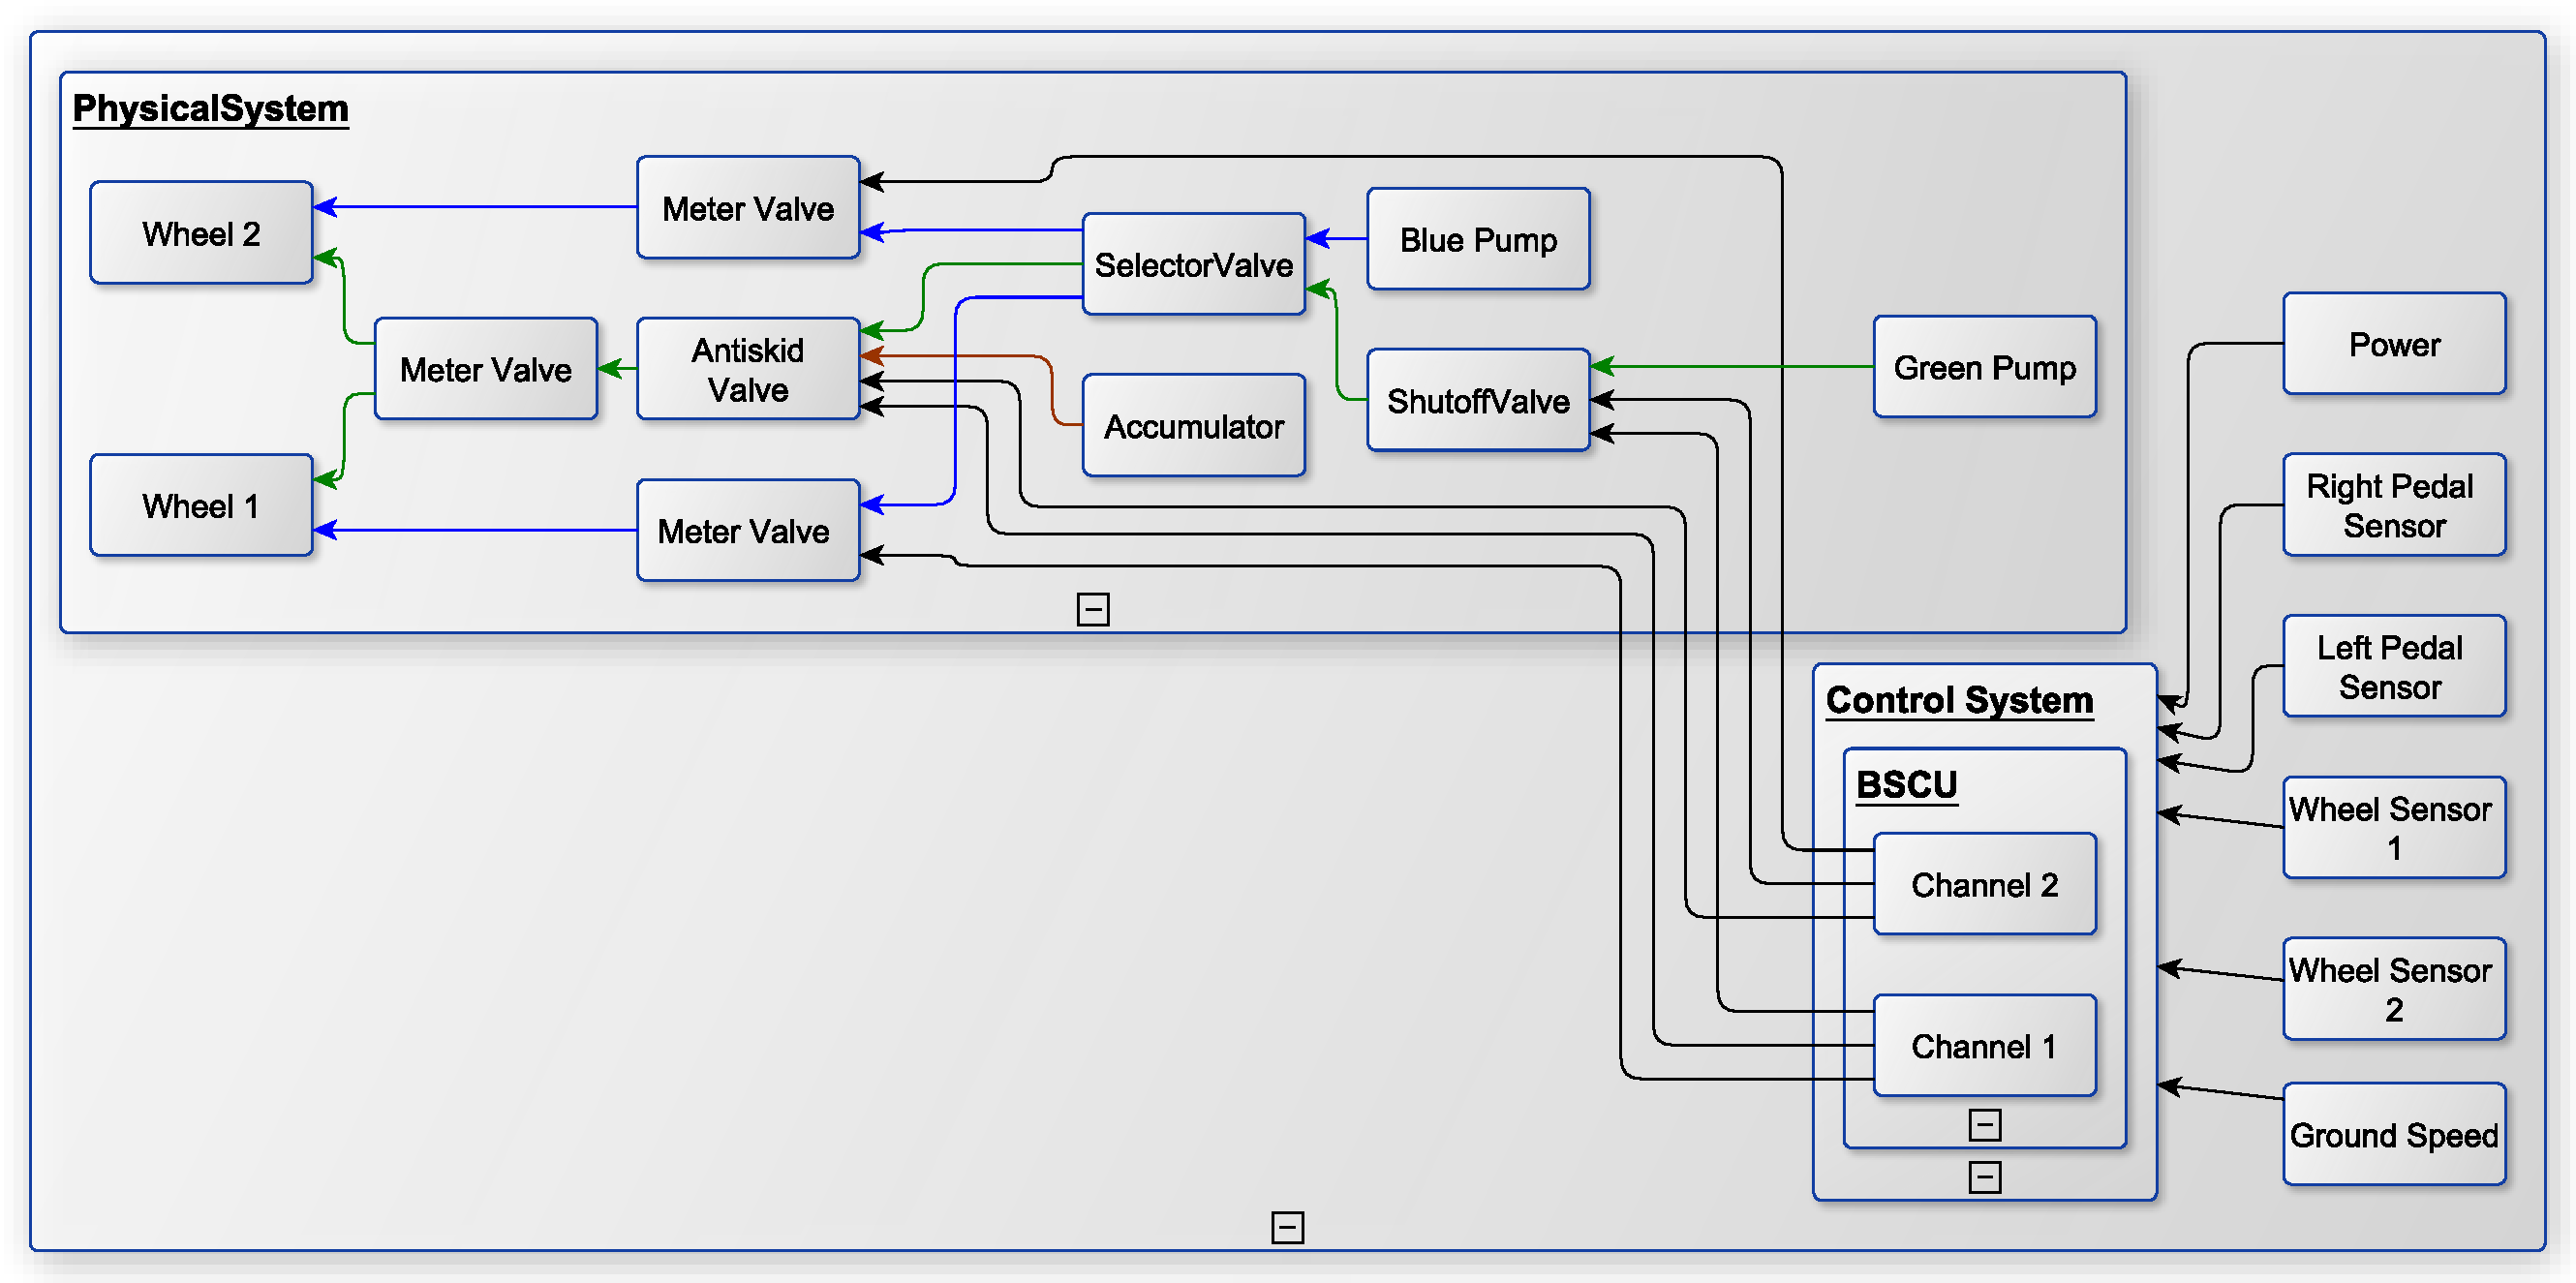
\includegraphics[trim=0 9 0 5,clip,width=\textwidth]{images/wbs_arch4_diagram.pdf}
	\caption{Wheel Brake System}
	\label{fig:wbs}
\end{figure} 

The model contains 30 different kinds of components, 169 component instances, a model depth of 5 hierarchical levels.  The model includes one top-level assumption and  27 top-level system properties, with 113 guarantees allocated to subsystems.  There are a total of 33 different fault types and 141 fault instances within the model.  The large number of fault instances is due to the redundancy in the system design and its replication to control 8 wheels. 

An example system safety property is to ensure that there is no inadvertent braking of any of the wheels. This is based on a failure condition described in AIR6110 is \textit{Inadvertent wheel braking on one wheel during takeoff shall be less than 1E-9 per takeoff}. 
Inadvertent braking means that braking force is applied at the wheel but the pilot has not pressed the brake pedal.  In addition, the inadvertent braking requires that power and hydraulic pressure are both present, the plane is not stopped, and the wheel is rolling (not skidding). 
%in Figure~\ref{fig:inadvertent_braking}. 
The property is stated in AGREE such that inadvertent braking does \textit{not} occur, as shown below. 

\begin{figure}[h!]
	\vspace{-0.2in}
	\begin{center}
		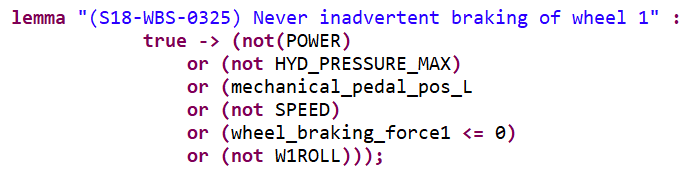
\includegraphics[width=.7\textwidth]{images/inadvertent_braking.png}
	\end{center}
	\vspace{-0.3in}
	%\caption{AGREE Contract for Top Level Property}
	\label{fig:inadvertent_braking}
	%\vspace{-0.2in}
\end{figure}

\subsubsection{Fault Analysis of WBS using Safety Annex}

The fault analysis on the top level WBS system was performed on the 11 top-level properties applying the max fault hypothesis and probabilistic fault hypothesis separately. It requires between 2 and 4 minutes to run either compositional analysis with max fault hypothesis or monolithic analysis with probabilistic fault hypothesis on the model. The analysis is computationally inexpensive, allowing quick iterations between systems and safety engineers.

We first applied compositional analysis with max one fault hypothesis at all layers of the model. Most properties were verified except for the \textit{Inadvertent braking at the wheel} properties. The failure of the verification for those properties shows that they are not resilient to a single fault. We then applied monolithic analysis with probabilistic fault hypothesis of $10^{-9}$ fault threshold. The \textit{Inadvertent braking at the wheel} properties also failed. Results from the first round of checks indicate that the WBS design is not fault tolerant to the inadvertent braking properties and is not meeting the Probability of Failure goal of $10^{-9}$ on those properties.

The counterexample returned by the tools allowed us to straightforwardly diagnose the fault conditions that lead to property failure: in this model, there is a single pedal position sensor for the brake pedal. If this sensor fails, it can command braking without a pilot request. The counterexample can be used to further analyze the system design and explore a solution to the problem. There are several ways to proceed (here we note that the architecture of the pedal assembly is not discussed in AIR6110):
	\begin{itemize}
	\renewcommand{\labelitemi}{\textbullet}
	\item Decrease the probability of failures of the brake pedal sensor. The failure probabilities are estimated from the failure rates and exposure times of the events. We may adjust the exposure time to match the phase of flight, rather than normalizing it per-flight-hour, if the phase of flight is sufficiently short. We may also find a brake pedal sensor with a lower failure rate. For example, if the failure probability for the sensor component is lower than the $10^{-9}$ fault threshold, it will not be considered in the possible fault combinations for the analysis. Decreasing the probability of failure of the components could help increase the reliability of the system. However, in this case the system still has a single point of failure.

	\item Create redundancy in the sensor component and model a voting procedure.
	In order for braking to occur, both (or all) sensors must agree. This would eliminate a single point of failure and would also cause the model to meet the top level probabilistic threshold. However, by introducing redundancy, it could affect the probability of meeting of other properties in the system that command braking, for example, when braking is commanded, braking pressure is provided at the wheel. Introducing the redundancy can increase the integrity of the system with respect to inadvertent braking, but decrease the availability of the system with respect to braking when needed.
\end{itemize}

Providing a way to quickly and effectively run analysis on the model 
for these different modes of failure can be of great benefit to assist system engineers to make design decisions and safety engineers to assess the effect.


\subsection{Quad-Redundant Flight Control System}
We have also used the Safety Annex to examine more complex fault types, such as asymmetric (or {\em Byzantine}) faults.  A Byzantine fault presents different symptoms to different observers, so that they may disagree regarding whether a fault is present.
We extended the Quad-Redundant Flight Control System (QFCS) example~\cite{QFCS15:backes} to model and analyze various types of faulty behaviors. Faulty behaviors were introduced to analyze the response of the system to multiple faults, and to evaluate fault mitigation logic in the model. As expected, the QFCS system-level properties failed when unhandled faulty behaviors were introduced.

We also used the Safety Annex to explore more complicated faults at the system level on a simplified QFCS model with cross-channel communication between its Flight Control Computers.

\begin{itemize}
	\item Byzantine faults~\cite{Driscoll-Byzantine-Fault} were simulated by creating one-to-one connections from the source to multiple observers so that disagreements could be introduced by injecting faults on individual outputs. The system level property ``at most one flight control computer in command'' was falsified in one second in the presence of Byzantine faults on the baseline model. The same property was verified in three seconds on an extended model with a Byzantine fault handling protocol added.  System designers can use this approach to verify if a system design is resilient to Byzantine faults, examine vulnerabilities, and determine if a mitigation mechanism works.

%original wording:	
	% A system-level property failed due to the fault on the baseline model, but did not fail on the model with Byzantine fault handling protocol added. Using the Safety Annex like this can test a system's vulnerability to Byzantine faults and verify mitigation mechanisms.
	
	\item Dependent faults were modeled by first injecting failures to the cross-channel data link (CCDL) bus (physical layer), and faults to the flight control computer (FCC) outputs (logical layer), then specifying fault propagations in the top level system implementation (where the data connections between FCC outputs were bound to the CCDL bus subcomponents). The fault propagation indicates that one CCDL bus failure can trigger all FCC output faults. With the fault hypothesis that allows a maximum of one fault active during execution, the system level property ``not all FCCs fail at the same time'' was falsified in one second.
	
%original wording:
%Dependent faults were modeled by injecting failures to hardware components (physical layer), and faults to software components (logical layer) that are bound to the hardware components, then specifying fault propagations at the QFCS system level to indicate that the software faults are dependent on the hardware failures. 	
\end{itemize}

%\mike{Results?} \janet{updated the last two paragraphs}
